\documentclass[border=10pt]{standalone}
\usepackage{tikz}\usepackage{amsmath}\usepackage{amssymb}\usetikzlibrary{calc,arrows.meta}
\begin{document}
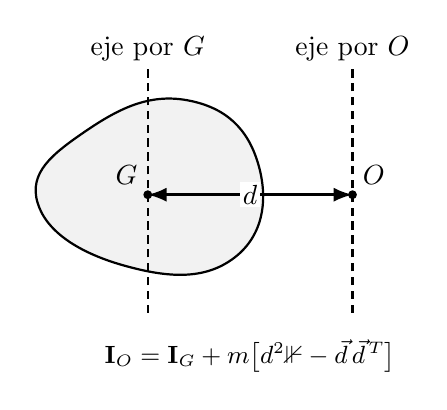
\begin{tikzpicture}[line width=0.9pt,>={Latex[length=2.4mm]}]
  \draw[thick,fill=black!5] plot[smooth cycle,tension=0.8] coordinates {(-1.0,0.9)(0.3,1.3)(1.2,0.5)(0.9,-0.7)(-0.5,-0.8)(-1.6,0.0)};
  \coordinate (G) at (-0.2,0.1); \coordinate (O) at (2.4,0.1);
  % ejes perpendiculares al plano (por G y por O)
  \draw[densely dashed] ($(G)+(0,-1.5)$)--($(G)+(0,1.6)$);
  \draw[densely dashed] ($(O)+(0,-1.5)$)--($(O)+(0,1.6)$);
  \fill (G) circle(1.6pt); \node[above left] at (G){$G$};
  \fill (O) circle(1.6pt); \node[above right] at (O){$O$};
  \node at ($(G)+(0,1.85)$){eje por $G$}; \node at ($(O)+(0,1.85)$){eje por $O$};
  \draw[<->] (G)--(O) node[midway,fill=white,inner sep=1pt]{$d$};
  \node at (1.1,-1.95){\small $\mathbf I_O=\mathbf I_G+m\big[d^2\mathbb 1-\vec d\,\vec d^{\,T}\big]$};
\end{tikzpicture}
\end{document}
